\chapter{Implementierung}
In diesem Kapitel geht es um die eigentliche Entwicklung des Projekts. Die Recherchen von wichtigen und notwendigen Informationen, 
die Planungen des generellen Vorgehens, Struktur- sowie Architekturpläne wie die Implementierung vonstatten gehen soll und wie die 
Planungen im Endeffekt umgesetzt wurden.
\section{Use Case1: Startmenü}
\subsection{Frontend (Mikka Jenne)}
Nach der grundlegenden theoretischen Ausarbeitung der Softwarearchitektur, dem allgemeinen Aufbau und dem Design ging der praktische Abschnitt
dieser Arbeit los. Die zu Anfang definierten Use Cases wurden in logischer, aufeinander aufbauender Reihenfolge aufgestellt und in jeweils Front- und Backend Entwicklung
aufgeteilt. 
Die ersten Entwicklungsschritte waren das Implementieren der grafischen Benutzeroberfläche (GUI) des Startmenüs, um daraufhin das Backend passend zu dieser
Oberfläche zu erstellen. Somit wurde ersichtlich, welche Funktionen diese erste Benutzeroberfläche umfasst.
\\
\linebreak
Bei der Umsetzung der Startmenu-UI wurde sich an dem MockUp in Abbildung 4.3 orientiert, bzw. an die vorangestellten 
Überlegungen angelehnt.
Dabei wurde darauf geachtet, dass der Unterschied des Designs nur in feineren Details, z.B. den Identifizierungs-Icons von dem eigentlichen Objekt abweicht, um weiteren
Umstrukturierungen aus dem weg zu gehen.
\\Im Vergleich zur Abbildung 4.3 wurden die in Kapitel 4 genannten Anforderungen umgesetzt und so ein anwendungsfreundliches 
und übersichtliches Startfenster erzeugt. 
\\Das UserControl basierende XAML wurde mit einem Grid, welches in Kapitel 3 näher beschrieben ist, versehen und 
in drei Bereiche aufgeteilt. Zum einen die Rubrik zum Erstellen von neuen Projekten, die Rubrik zum Öffnen von vorhandenen Projekten und zum anderen 
die Rubrik zum Anzeigen von vorhandenen Projekten, die sich lokal auf dem Computer befinden.
\\Auf die Ansicht der Liste der vorhandenen Projekte wird im Nachgang in dem Code-Beispiel 5.1 noch genauer eingegangen.
\\Um das Aussehen für den Benutzer interessanter und anschaulicher zu gestalten wurde der Hintergrund des Fensters und diverse Maus-Highlighting-Effekte
mit Blautönen versehen. 
\\Die genannten Grid-Rubriken für das Erstellen und Öffnen von neuen Projekten wurde mit einem Button implementiert, um das 
jeweilige Event auslösen zu können und um auf die referenzierten Seiten zu gelangen. Diese Referenzierungen wurden anschließend im 
\textit{Backend} realisiert. 
\\Die folgende Abbildung repräsentiert das Aussehen des Startmenüs, wenn die Applikation gestartet, bzw. ausgeführt wird.
\\Nachdem dieses Objekt erstellt wurde, konnte mit der weiteren Entwicklung fortgefahren werden und unabhängig zu der Backend-Entwicklung 
dieses Use Cases ein weiteres benötigtes Benutzerfenster, die Eingabe eines Projektnamens für ein neues Projekt, erstellt werden.
\\
\begin{figure}[hbt!]
    \centering
    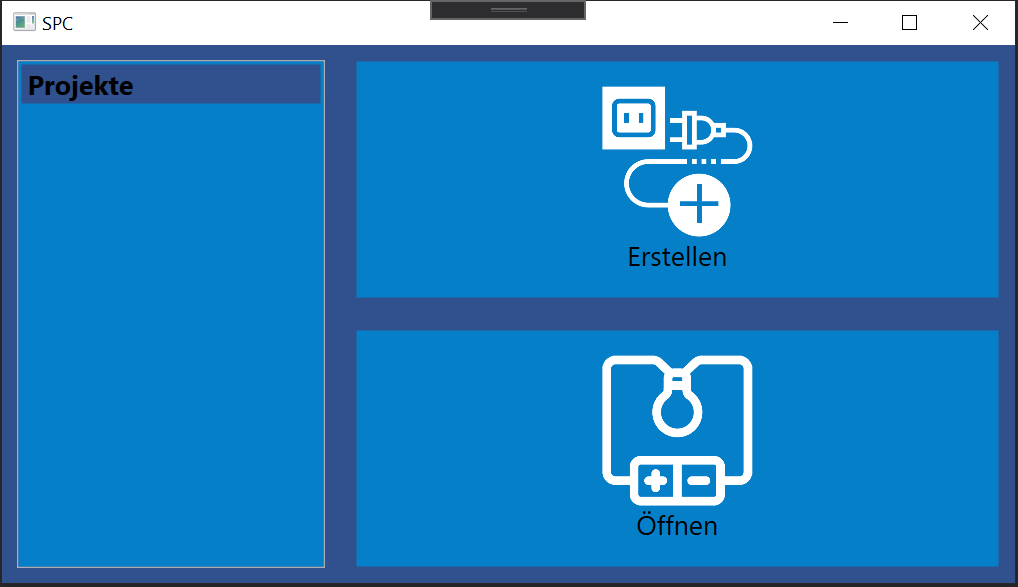
\includegraphics[width=15cm,height=10cm,keepaspectratio]{5Implementierungen/Bilder/StartMenuView.png}
    \caption{Startmenü View}
\end{figure}
\\
Um den Prozess, ein Projekt zu erstellen, fließend übergehen zu lassen wird zwischen der Startmenu-Seite und dem eigentlichen Editor eine zusätzliche
Komponente benötigt, die zwischen den Komponenten transferiert und alle benötigten Informationen von dem Benutzer einholt, benötigte Ressourcen generiert und lädt. 
\pagebreak
\\Beim betätigen des Erstellen-Buttons wird das UserControl der \textit{ProjektNameEingabeView}-Seite aufgerufen. In diesem Schritt der 
Applikation kann der Benutzer dem Projekt einen Namen vergeben und die Datei so im Verzeichnis anlegen. Die dazugehörige GUI beinhaltet eine 
schlichte und einfach gehaltene Eingabemaske, in der lediglich ein Textfeld zur Eingabe des Projektnamens vorhanden ist. Ebenso ist diese mit zwei Buttons versehen die jeweils 
den Prozess zum einen voranbringen durch den (\textit{WeiterButton}) oder zum anderen auf den vorherigen Stand zurückgehen, indem der (\textit{ZurueckButton}) gedrückt wird.
\\
\linebreak
\begin{figure}[htb!]
    \centering
    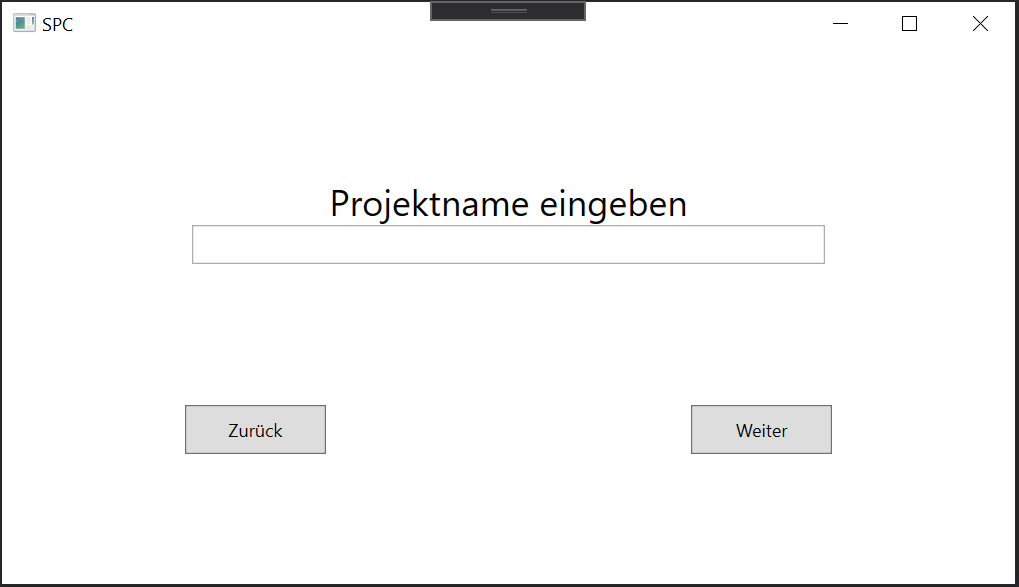
\includegraphics[width=15cm,height=10cm,keepaspectratio]{5Implementierungen/Bilder/ProjektNameEingabeView.png}
    \caption{Projektname View}
\end{figure} 
\pagebreak 
\\Der Code-Ausschnitt zeigt eine vereinfachte From des implementierten UserControls der Eingabe eines Projektnamens. Dabei wurde der \textit{Code behind} weggelassen, da 
in diesem Fall nur das Frontend-Design betrachtet wird. 
\\Dies kann der folgenden Abbildung entnommen werden.
\\
\begin{lstlisting}[language=XML,
    frame=single,           % Ein Rahmen um den Code
    framexleftmargin=15pt,  % Rahmen link von den Zahlen
    style=algoBericht,
    label={startmenuview},
    captionpos=b,           % Caption unter den Code setzen
caption={Projektname-View XAML-Code}]
<UserControl    
    DataContext="{Binding Main, Source={StaticResource Locator}}">
    <Grid>
        <Grid>
            <Grid.RowDefinitions>
                <RowDefinition/>
                <RowDefinition/>
                <RowDefinition/>
            </Grid.RowDefinitions>
            <Grid.ColumnDefinitions>
                <ColumnDefinition/>
                <ColumnDefinition/>
            </Grid.ColumnDefinitions>
            <TextBlock Text="Projektname eingeben" Grid.ColumnSpan="2" 
            FontSize="24" 
            TextAlignment="Center" 
            HorizontalAlignment="Center" VerticalAlignment="Bottom"/>
            <TextBox Grid.Column="0" x:Name="ProjektNameTextFeld"/>
            <Button Grid.Column="0"  x:Name="ZurueckButton" 
            Grid.Row="2" Content="Zurueck"/>
            <Button x:Name="WeiterButton" Grid.Row="2" 
            Grid.Column="1" Content="Weiter"/>
        </Grid>
    </Grid>
</UserControl>
\end{lstlisting}
Als Transferseite wurde diese vom Design unaufmerksam gehalten, da ein Benutzer in der Regel nicht viel Zeit auf dieser Seite aufwenden muss.
Nach dem Ausfüllen des Textblocks und der Bestätigung durch den \textit{WeiterButton} wird der Benutzer direkt auf den eigentlichen Editor weitergeleitet und ist somit in der 
Hauptansicht der eigentlichen Anwendung. 

\subsection{Backend (Simon Leitl)}
Für die Funktionalität des Startmenüs sind mehrere Klassen verantwortlich. Nach MVVM-Prinzip findet die Logik innerhalb der 
ViewModel-Klassen statt. Speziell für das Startmenü lassen sich die Funktionalitäten in drei Bereiche aufteilen.
\begin{itemize}
    \item Das erstellen eines neuen Projekts
    \item Die Anzeige der gespeicherten Projekte im automatisch generierten Projektordner  
    \item Das öffnen eines gespeicherten Projekts
\end{itemize}
Der Nutzer hat die Möglichkeit ein neues 
Projekt über die Schaltfläche \textit{Erstellen} zu erstellen. Hierbei muss im Hintergrund des 
Programms eine neue Datei angelegt werden. Die Datei wird später Daten enthalten, mit welchen die Schaltpläne gespeichert werden können. 
Da der Aufwand ein eigenes Dateiformat zu erstellen für diese Arbeit zu hoch wäre, wird das Textdatei (txt) Format verwendet. Dies eignet 
sich um die Daten der Zeichnung abzuspeichern. Mithilfe von Input/Output Streams ist es so möglich, die Daten in die Textdatei zu schreiben 
und zu lesen. Um die gespeicherten Projekte an einem gemeinsamen Ort abzulegen wird zunächst beim ersten Ausführen, automatisch ein Ordner 
erstellt. In diesem werden zukünftig die neu erstellten Projekte, also Textdateien, abgelegt. 
Um den gesamten Prozess zu starten wird im Startmenu \textit{Erstellen} ausgewählt. Von dort wird man innerhalb des Fensters 
weitergeleitet auf die Benutzeroberfläche ProjektNameEingabeView, welche die Möglichkeit bietet ein Projektname über das vorhandene 
Eingabefeld einzugeben. Über den Button \textit{weiter} wird das Projekt erstellt. Hierbei wird innerhalb der Logik ein RelayCommand 
ausgeführt. Dieser kommuniziert die Interaktion über das, in der XAML festgelegten, Binding. Die Logik wird in der 
ProjektnameEingabeViewModel Klasse als Methoden abgebildet und ausgeführt. Wird also mit dem Button \textit{weiter} interagiert, 
so wird die Methode \textit{NewProjektCommand} im folgenden Code \refname{NewProjektCommand} aufgerufen. 
\linebreak
\begin{lstlisting}[language=C,
    frame=single,           % Ein Rahmen um den Code
    framexleftmargin=15pt,  % Rahmen link von den Zahlen
    style=algoBericht,
    label={NewProjektCommand},
    captionpos=b,           % Caption unter den Code setzen
    caption={NewProjektCommand}]
    public RelayCommand NewProjektCommand { get; private set; }
\end{lstlisting}
Über die enthalten get Methode wird die Interaktion übergeben. Der RelayCommand selbst ruft eine weitere Methode zur Ausführung auf.
\\
\begin{lstlisting}[language=C,
    frame=single,           % Ein Rahmen um den Code
    framexleftmargin=15pt,  % Rahmen link von den Zahlen
    style=algoBericht,
    label={CreateNewProject},
    captionpos=b,           % Caption unter den Code setzen
    caption={CreateNewProject}]
    public void CreateNewProject()
        {
            if (CheckProjectDirectory() == true)
            {
                CreateProjectFile();
            }
            else
            {
                CreateProjectDirectory();
                CreateProjectFile();
            }
        }

\end{lstlisting}
Die Methode \textit{CreateNewProject} ist der Startpunkt der Ablauffolge um eine neues Projekt und damit eine neue Datei zu erstellen. 
Es überprüft zunächst ob der Ordner, in dem die Dateien erzeugt werden sollen, vorhanden ist. Dies gelingt über eine if-Abfrage, die den 
boolschen zurückgegebenen Wert einer Methode auf Richtigkeit überprüft. Bei der Methode handelt es sich um die nachfolgende Methode mit 
dem Namen \textit{CheckProjectDirectory}. Sie gibt \textit{true/false} als Ausgabe zurück. Der Ordner für gespeicherte Dateien, sollte 
sich im selben Pfad bzw. Ablageort befinden wie die ausführende kompilierte .exe des Programms. 
\pagebreak
\begin{lstlisting}[language=C,
    frame=single,           % Ein Rahmen um den Code
    framexleftmargin=15pt,  % Rahmen link von den Zahlen
    style=algoBericht,
    label={CheckProjectDirectory},
    captionpos=b,           % Caption unter den Code setzen
    caption={CheckProjectDirectory}]
    public Boolean CheckProjectDirectory()
    {
       return Directory.Exists("Savings");
    }

\end{lstlisting}
Ist der Rückgabewert \textit{true} wird eine weitere Methode \textit{CreateProjectFile} ausgeführt. Diese enthält Funktionen zum 
erstellen der Datei. Wird \textit{false} zurückgegeben, ist das Verzeichnis nicht vorhanden und muss mittels der Methode 
\textit{CreateProjectDirectory} erstellt werden. 
\\
\begin{lstlisting}[language=C,
    frame=single,           % Ein Rahmen um den Code
    framexleftmargin=15pt,  % Rahmen link von den Zahlen
    style=algoBericht,
    label={CreateProjectDirectory},
    captionpos=b,           % Caption unter den Code setzen
    caption={CreateProjectDirectory}]
    public void CreateProjectDirectory()
        {
            Directory.CreateDirectory("Savings");

        }
\end{lstlisting}
CreateProjectDirectory nutzt System.IO.Directory für 
das Erstellen des Verzeichnisses. Das Verzeichnis soll mit dem Namen 
\textit{Savings} erstellt werden. 
\linebreak
Jetzt wurde sichergestellt, dass das Verzeichnis zum speichern der Dateien existiert und verfügbar ist. Im nächsten Schritt wird die 
Datei erzeugt. Hierfür dient die \textit{CreateProjectFile} Methode. Zunächst wird allerdings der vom Benutzer gewählte Projektname 
benötigt. Dieser kann über die  Benutzereingabe erlangt werden. Hierfür wurde eine weitere Methode implementiert, welche an die View gebindet wurde. 
\\
\begin{lstlisting}[language=C,
    frame=single,           % Ein Rahmen um den Code
    framexleftmargin=15pt,  % Rahmen link von den Zahlen
    style=algoBericht,
    label={ProjektName},
    captionpos=b,           % Caption unter den Code setzen
    caption={ProjektName}]
    public string ProjektName
    {
        get { return projektName; }
        set { projektName = value; }
    }
\end{lstlisting}
Sie gibt den Eingabewert des Nutzer zurück und speichert ihn in einer globalen Variable \textit{projektName}. Diese Variable wird 
im folgenden dazu verwendet die Datei mit dem eingegebenen Namen zu erzeugen.
\\
\begin{lstlisting}[language=C,
    frame=single,           % Ein Rahmen um den Code
    framexleftmargin=15pt,  % Rahmen link von den Zahlen
    style=algoBericht,
    label={ProjektName},
    captionpos=b,           % Caption unter den Code setzen
    caption={ProjektName}]
    public void CreateProjectFile()
    {
        String path = "Savings/" + projektName + ".txt";
        using (FileStream fs = File.Create(path)){}
        MainEditorWindowView mw = new MainEditorWindowView();
        mw.Show();
    }
\end{lstlisting}
Im ersten Schritt der Methode wird der Pfad definiert, der 
benötigt wird um die Datei abzulegen. Hierbei wird der 
Name des Verzeichnis angegeben sowie der Name des Projekts und die Dateiendung. Über einen \textit{Filestream} wird dann die Datei, 
mit dem zuvor festgelegten Pfad erzeugt. Da dies der abschließende Schritt beim Erstellen eines neuen Projektes war, muss das die 
nächster Benutzeroberfläche geladen werden. Es handelt es sich um den Editor. Eine neue Instanz des MainEditorWindowView wird erstellt 
und durch den Befehl \textit{Show()} geöffnet. 
\linebreak
\linebreak
Die zweite Funktion des Startmenü beinhaltet die Anzeige der gespeicherten Projekte. Sie soll einen schnellen Zugriff auf die 
vorhandenen Projekte gewährleisten. Hierzu werden die Projektdateien in Form einer Liste untereinander ausgegeben. Für die 
Implementierung dieser Funktion müssen also alle Dateien, die innerhalb des Verzeichnis liegen, abgerufen und auf der 
Benutzeroberfläche ausgegeben werden. Da es Möglich ist ganze Listen an die View zu binden, werden die Dateinamen in einer Liste 
gespeichert. Die Implementierung befindet sich in der MainViewModel-Klasse des Startmenü. 
\\
\begin{lstlisting}[language=C,
    frame=single,           % Ein Rahmen um den Code
    framexleftmargin=15pt,  % Rahmen link von den Zahlen
    style=algoBericht,
    label={showProjekte},
    captionpos=b,           % Caption unter den Code setzen
    caption={showProjekte}]
        public void showProjekte()
        {
            string path = @"\Savings";
            
            ProcessDirectory(path);
            splitString();
        }
\end{lstlisting}
In der Methode \textit{showProjekte} ist zunächst der Pfad für den Ort des Verzeichnis deklariert. Mit diesem wird eine weitere 
Methode \textit{ProcessDirectory(path)} aufgerufen. Durch diese Methode werden alle Dateien innerhalb des Verzeichnis in eine Liste 
geschrieben. 
\\
\begin{lstlisting}[language=C,
    frame=single,           % Ein Rahmen um den Code
    framexleftmargin=15pt,  % Rahmen link von den Zahlen
    style=algoBericht,
    label={ProcessDirectory},
    captionpos=b,           % Caption unter den Code setzen
    caption={ProcessDirectory}]
    public void ProcessDirectory(string targetDirectory)
    {
        // Process the list of files found in the directory.
        string[] fileEntries = Directory.GetFiles(targetDirectory);

        foreach (string fileName in fileEntries)  
        filePaths.Add(fileName);                  
    }
\end{lstlisting}
Über die in System.IO enthalten Methode \textit{Directory.GetFiles(Path)} werden alle Dateien die innerhalb des zuvor definierten Pfad liegen, ausgegeben. Hier werden diese gleich in einen Array \textit{fileEntries} gespeichert. Mithilfe einer Schleife werden die einzelnen Dateinamen in eine weitere Liste \textit{filePaths} geschrieben, welche global definiert wurde. Da die Methode den vollständigen Dateipfad und nicht nur den Namen der Datei ausgibt, muss der \textit{String} zerteilt werden. Dafür wird der String im nachfolgenden Code gesplittet. 
\pagebreak
\begin{lstlisting}[language=C,
    frame=single,           % Ein Rahmen um den Code
    framexleftmargin=15pt,  % Rahmen link von den Zahlen
    style=algoBericht,
    label={splitString},
    captionpos=b,           % Caption unter den Code setzen
    caption={splitString}]
    public void splitString()
        {
            for (int i = 0; i < filePaths.Count; i++){
                string name = filePaths[i];
                string[] split = Regex.Split(name, "\\");
                _files.Add(split[split.Length-1]);
                }
        }
\end{lstlisting}
Die Liste \textit{filePaths}, welche Global definiert wurde und die Dateipfade beinhaltet wird hier über \textit{Regex.Split()} aufgeteilt. Die Bedingung für die Aufteilung ist der sogenannte Backslash \textbackslash. Jedesmal wenn innerhalb der Zeichenkette ein Backslash erscheint, wird an dieser Stelle geteilt und als neue Position in die Liste geschrieben. Da der Dateiname der letzte Teil des Pfads ist, kann der letzte Eintrag der Liste als Dateinamen ausgewählt werden. Damit alle Einträge der Liste gesplittet und in die neue Liste \textit{files} eingetragen werden, wird in einer Schleife über die Liste iteriert. \textit{files} wird in der folgenden Methode dazu genutzt um an die View anhand eines Bindings übergeben zu werden. 
\\
\begin{lstlisting}[language=C,
    frame=single,           % Ein Rahmen um den Code
    framexleftmargin=15pt,  % Rahmen link von den Zahlen
    style=algoBericht,
    label={getFileList},
    captionpos=b,           % Caption unter den Code setzen
    caption={getFileList}]
    public ObservableCollection<string> getFileList
    {
        get
        {
            return _files;
        }
    }
\end{lstlisting}
Die Methode \textit{getFileList} liefert die Liste mit den Dateinamen als Observablecollection zurück. Das UI Element kann über ein Binding zu dieser Methode die Namen auf der Benutzeroberfläche abbilden.  
Ein Code-Ausschnitt der Listenansicht-Implementierung soll einen Einblick verschaffen wie die \textit{Starmenu-XAML} in Bezug auf die Liste aufgebaut und 
Über die in System.IO enthalten Methode \textit{Directory.GetFiles(Path)} 
werden alle Dateien die innerhalb des zuvor definierten Pfad 
liegen, ausgegeben. Hier werden diese gleich in einen Array \textit{fileEntries} gespeichert. Mithilfe einer Schleife werden die einzelnen 
Dateinamen in eine weitere Liste \textit{filePaths} geschrieben, welche global definiert wurde.
\\
Ein Code-Ausschnitt der Listenansicht-Implementierung soll einen Einblick verschaffen wie die 
\textit{Starmenu-XAML} in Bezug auf die Liste aufgebaut und 
implementiert ist.
\\
\pagebreak
\section{Use Case 2: Toolbox}
Nachdem die Dateien und Objekte zur Erstellung eines Projekts implementiert waren, wurde sich dem Frontend des Editors gewidmet, um die eigentlichen
Funktionen bereitzustellen, damit die Implementierung des Editors umgesetzt werden konnte. 
\\Parallel zu dem Design des Startmenüs wurden ebenso die grafische Darstellung 
des Editors erstellt. Das dazugehörige MockUp wurde in Kapitel 4 Abbildung 4.4 bereits erwähnt und genauestens beschrieben. 
Da die Überlegungen zum Design im Voraus getätigt und eine visuelle Vorarbeit geleistet wurde, konnte sich bei der Entwicklung lediglich an dem 
grafisch dargestellten Entwurf orientiert werden.
\subsection{Frontend (Mikka Jenne)}
Das UI-Element des Editors besteht grundlegend aus einem \textit{Window-XAML} und ist in ein Raster aufgeteilt. Um das Raster zu verdeutlichen, wird die Definition dieses Rasters aufgeführt.
\\ 
\begin{lstlisting}[language=XML,
    frame=single,           % Ein Rahmen um den Code
    framexleftmargin=15pt,  % Rahmen link von den Zahlen
    style=algoBericht,
    label={usercontrolsnippet},
    captionpos=b,           % Caption unter den Code setzen
caption={Editor Raster-Layout}]
<Grid.ColumnDefinitions>
    <ColumnDefinition/>
    <ColumnDefinition/>
    <ColumnDefinition/>
    <ColumnDefinition/>
    <ColumnDefinition/>
    <ColumnDefinition/>
    <ColumnDefinition/>
    <ColumnDefinition/>
</Grid.ColumnDefinitions>
<Grid.RowDefinitions>
    <RowDefinition Height="0.3*"/>
    <RowDefinition/>
    <RowDefinition/>
    <RowDefinition/>
    <RowDefinition/>
    <RowDefinition/>
    <RowDefinition/>
    <RowDefinition/>
</Grid.RowDefinitions>
\end{lstlisting}
Mit dieser Implementierung wird das \textit{Window} in ein Raster aufgeteilt mit Rechtecken gleicher Größe. Durch Verschmelzung einzelner Rechtecke können 
größere Flächen gebildet werden, um dementsprechend mehr Inhalt darin anzeigen zu können. So kann z.B. ein \textit{UserControl} referenziert werden,
welches viel Platz benötigt. In dem Fall des Editors ist das die eigentliche Zeichenfläche.
\\ 
\\Das Editor-Element ist als ein separates 
\textit{Window} angelegt. Es öffnet sich nach dem betätigen des \textit{WeiterButton} des \textit{UserControls-ProjektNameEingabe} ein neues Fenster mit der Editor Ansicht. 
Auf diesen Schritt wird nicht weiter drauf eingegangen, da diese Aktion über das Backend verwaltet wird. 
\pagebreak
\\Der aktuelle Entwurf des Editors ist in folgender Abbildung zu entnehmen. Die Umsetzung ähnelt der Abbildung 4.4 in grundlegenden Struktur.
\begin{figure}[hbt!]
    \centering
    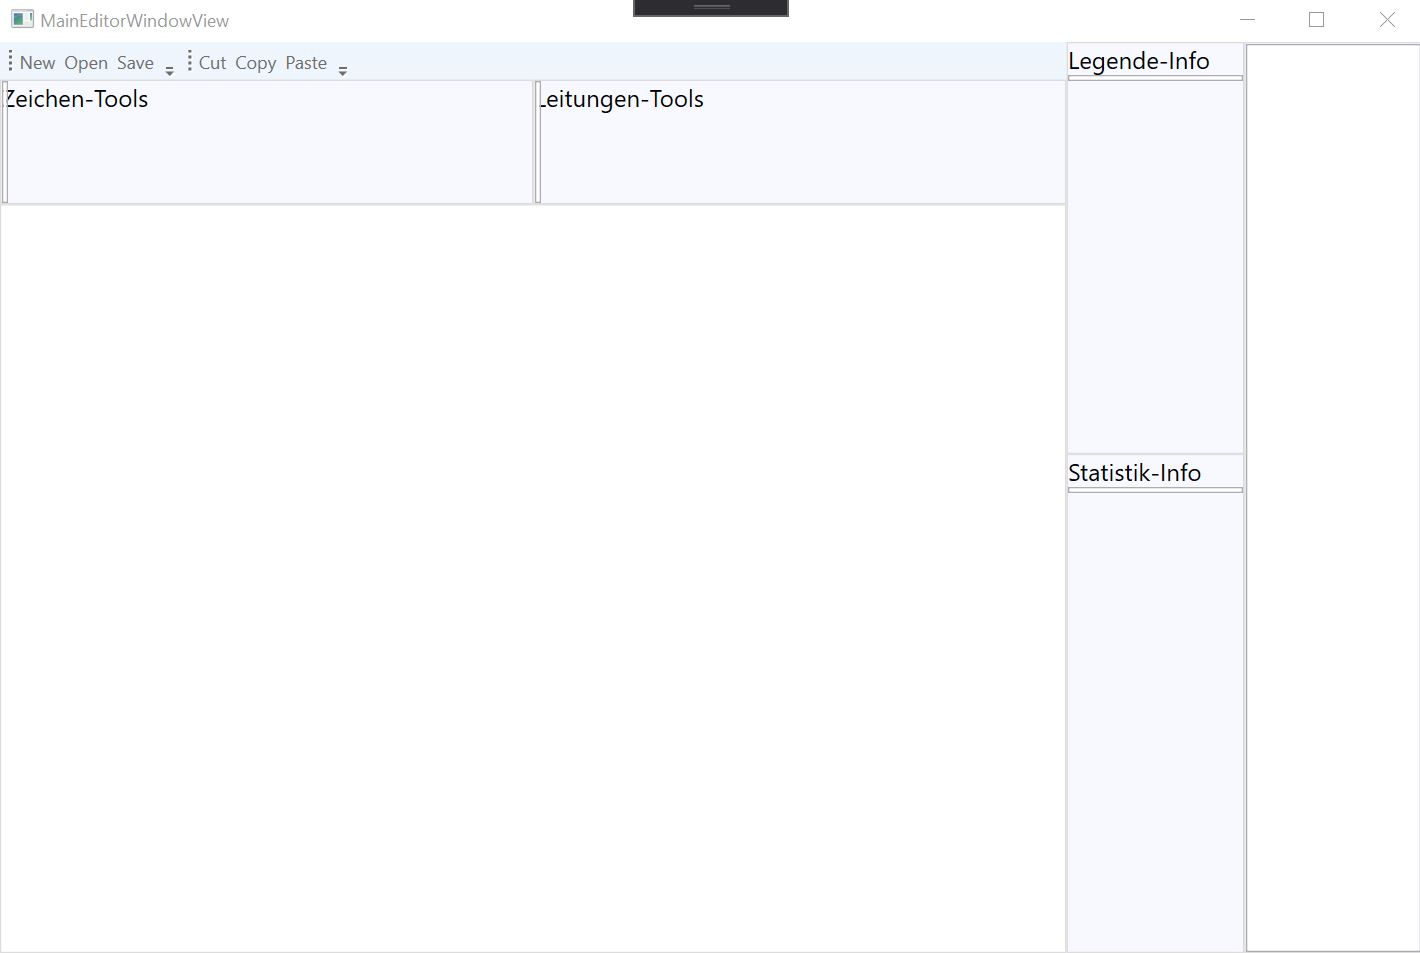
\includegraphics[width=15cm,height=10cm,keepaspectratio]{5Implementierungen/Bilder/EditorView.JPG}
    \caption{Editor View}
\end{figure}
\\Die \textit{Window}-Datei ist durch eine Anreihung von \textit{Grid-Elementen} strukturiert und in sieben unterschiedlich große Flächen gegliedert. Die 
Rasterelemente sind für eine jeweilige Komponente als Platzhalter gedacht, bzw. für ein bestimmtes \textit{UserControl} vorgemerkt. Alle Komponenten 
sind als ein \textit{UserControl} ausgelagert, um die Code-Struktur der Hauptseite zu entlasten und übersichtlicher zu gestalten.
\\Das \textit{Window-XAML}-Element is so als zentraler Ort für alle \textit{UserControls} bestimmt.
\\
\pagebreak
\\In folgender Abbildung wird die Aufteilung der einzelnen Felder in der \textit{XAML}-Datei veranschaulicht.
Um genauer zu verdeutlichen wie die einzelnen \textit{UserControls} in dem Editor-Fenster integriert werden, wird ergänzend zu der Abbildung 5.3 ein Code-
Ausschnitt von einer der \textit{UserControls} aufgeführt.
\\
\begin{lstlisting}[language=XML,
    frame=single,           % Ein Rahmen um den Code
    framexleftmargin=15pt,  % Rahmen link von den Zahlen
    style=algoBericht,
    label={usercontrolsnippet},
    captionpos=b,           % Caption unter den Code setzen
caption={UserControl-Referenz Code-Auschnitt}]
<Window
    xmlns:local="clr-namespace:SPC3.SPC.Editor.Views">
    <DockPanel Grid.Column="0" Grid.Row="2" 
     Grid.RowSpan="6" Grid.ColumnSpan="6">
        <Grid>
            <local:ZeichenFlacheView x:Name="ZeichenFlaecheView"/>
        </Grid>
    </DockPanel>
</Window>
\end{lstlisting}
Der Verweis durch \textit{local} gibt Informationen darüber in welchem Namespace oder genauer in welchem Ordner des Projekts dieses Objekt zu finden ist, um das Element 
referenzieren zu können. Durch diesen Aufruf wird dem Hauptfenster eindeutig mitgeteilt welche Klasse, konkret welches \textit{UserControl} in diesem Feld 
geladen werden soll.
Auf diese Weise werden alle \textit{UserControls} in die \textit{MainWindow-XAML}-Datei geladen.

\begin{lstlisting}[language=XML,
    frame=single,           % Ein Rahmen um den Code
    framexleftmargin=15pt,  % Rahmen link von den Zahlen
    style=algoBericht,
    label={startmenuview},
    captionpos=b,           % Caption unter den Code setzen
caption={Startmenu-Recent-Projects-Code}]
<ListView Grid.Column="0" x:Name="viewUsedProjects" Background="#067FC9" 
    Margin="10">
    <ListView.ItemTemplate>
        <DataTemplate>
            <WrapPanel>
                <TextBlock Text="{Binding ProjektPfad}"></TextBlock>
            </WrapPanel>
        </DataTemplate>
    </ListView.ItemTemplate>
    <ListViewItem Background="#31508E" FontWeight="Bold" FontSize="18">
    Projekte</ListViewItem>
</ListView>
\end{lstlisting}
Das ListView-Item wird eindeutig einer \textit{Grid.Column} zugeordnet und mit einer \textit{Background-Color} Farbe versehen. 
Zusätzlich wird dem Element
einen Namen vergeben, um bei einer Referenzierung das Objekt eindeutig ansprechen zu können.
\\Der Ausschnitt zeigt, wie der Aufruf, bzw. das \textit{Binding} eines Objekts, in dem Fall das dynamisch generierte \textit{ListView-Item}, 
angebunden und auf den Code im Backend verwiesen wird. 
\pagebreak
\subsection{Backend (Simon Leitl)}
Die Toolbox-Werkzeug beeinhalten, wie bereits innerhalb dieser Arbeit erwähnt, Funktionen und Komponten die nötig sind um den Schaltplan zu zeichnen. Der Aufbau der Elemente innerhalb der Toolboxen wird im folgenden Abschnitt exemplarisch anhand der Elektronischen Komponenten erläutert. 
\begin{figure}[hb]
    \centering
    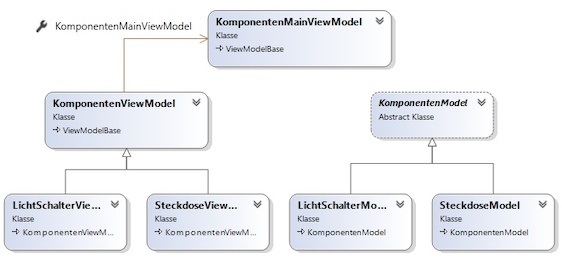
\includegraphics[width=500px,height=193px]{5Implementierungen/Bilder/ClassDiagram1}
    \caption{Klassendiagramm Toolbox}
    \label{pic:klassendiagramm-toolbox}
\end{figure}
\linebreak
Das oberhalb abgebildetet Klassendiagramm gibt die Klassen, welche die Komponenten repräsentieren wieder. Auch hier lassen sich wieder Models und ViewModels gemäß MVVM wiederfinden. Dabei enthalten die Models die Struktur einer Komponente. In diesem Fall den Namen der Komponenten, sowie Eigenschaften des Symbols. Die ViewModels dienen dazu die Struktur der KomponentenModels abzubilden und mit einer Logik zu versehen. Außerdem werden die einzelnen Komponenten später über die ViewModels aufgerufen, da nicht direkt mit den Models kommuniziert wird. Denn diese sollen nur die Datenstruktur festlegen.
In diesem Beispiel werden zwei Komponenten behandelt. Ein Lichtschalter und eine Steckdose sollen zur Verfügung gestellt werden. Diese sollen später in den Schaltplan integriebar sein. Beide Klassen, LichtSchalterModel und SteckdoseModel erben von der abstrakten Klasse KomponentenModel. Die abstrakte Klasse gibt die allgemeine Struktur für die Models der Komponenten vor. Wenn eine weitere Komponente hinzugefügt werden soll, muss jediglich ein Model erstellt werden, das von der abstrakten KomponentenModel Klasse erbt. Die Methoden und Eigenschaften sind dann aufgrund der Vererbung vorgegeben. Somit gelingt eine einfache Erweiterung.
\pagebreak
\begin{lstlisting}[language=C,
    frame=single,           % Ein Rahmen um den Code
    framexleftmargin=15pt,  % Rahmen link von den Zahlen
    style=algoBericht,
    label={KomponentenModel},
    captionpos=b,           % Caption unter den Code setzen
    caption={KomponentenModel}]
    abstract class KomponentenModel
    {
        public KomponentenModel(){}

        public String komponentenName;
        private String komponentenBeschreibung;
        private String symbolPfad;

        public String KomponentenName
        {
            get -> komponentenName;
            set -> komponentenBeschreibung = value;
        }


        public String KomponentenBeschreibung
        {
            get -> komponentenBeschreibung;
            set -> komponentenBeschreibung = value;
        }

        public String symbolPfad
        {
            get -> symbolpfad;
            set -> symbolPfad = value;
        }
    }
\end{lstlisting}
Der konkrete Aufbau für eine KomponentenModel Klasse kann dem Code-Beispiel 5.15 entnommen werden. Es werden zunächst die Eigenschaften als drei globale Felder in Form von \textit{String} deklariert. Sie enthalten den Namen, eine Beschreibung und den Pfad zur Bilddatei der Komponente. Über öffentliche Getter- und Settermethoden ist es Möglich die Eigenschaften zu setzen und zu lesen. Es wird allerdings nicht empfohlen die Eigenschaften innerhalb des Systems zu ändern. Eine Änderung wird nur innerhalb der Modelklasse empfohlen. Die Methode wird jedoch implementiert um sie in möglichen Fällen bereitzustellen. 
\pagebreak
\begin{lstlisting}[language=C,
    frame=single,           % Ein Rahmen um den Code
    framexleftmargin=15pt,  % Rahmen link von den Zahlen
    style=algoBericht,
    label={KomponentenModel},
    captionpos=b,           % Caption unter den Code setzen
    caption={KomponentenModel}]
    class LichtSchalterModel : KomponentenModel
    {
      private string komponentenName = "Lichtschalter";
      private string symbolPfad = @"\KomponentenPictures\lichtschalter.png";

      public string getKomponentenName()
      {
          return komponentenName;
      }

      public string getSymbolPfad()
      {
          return symbolPfad;
      }
    }
\end{lstlisting}
Im Code-Beispiel 5.16 ist die konkrete Ausführung einer KomponentenModel Klasse dargestellt. Hier wird der Name, sowie der Symbolpfad festgelegt. Mithilfe von Gettermethoden werden diese zurückgegeben und bereitgestellt, sodass sie von den ViewModels im benutzt und implementiert werden können.
\begin{lstlisting}[language=C,
    frame=single,           % Ein Rahmen um den Code
    framexleftmargin=15pt,  % Rahmen link von den Zahlen
    style=algoBericht,
    label={LichtSchalterViewModel},
    captionpos=b,           % Caption unter den Code setzen
    caption={LichtSchalterViewModel}]
    public class LichtSchalterViewModel : KomponentenViewModel
    {
        LichtSchalterModel lichtSchalterModel = new LichtSchalterModel();
        public LichtSchalterViewModel()
        {
            Name = lichtSchalterModel.getKomponentenName();
            Symbol = lichtSchalterModel.getSymbolPfad();
        }
    }
\end{lstlisting}
Parallel zur Model Klasse einer Komponente, in diesem Fall der Steckdose, gibt es eine ViewModelKlasse der Komponente. Diese trägt den Klassennamen LichtSchalterViewModel. Sie implementiert, die im nachfolgenden Code-Beispiel 5.18 beschriebene KomponentenViewModel Klasse. Um die Daten der Model Klasse zu nutzen bildet die LichtSchalterViewModel Klasse eine Instanz ihrer zugehörigen Model Klasse. Mit dieser Instanz werden die Daten anhand der definierten Gettermethoden abgerufen. 
\pagebreak
\begin{lstlisting}[language=C,
    frame=single,           % Ein Rahmen um den Code
    framexleftmargin=15pt,  % Rahmen link von den Zahlen
    style=algoBericht,
    label={KomponentenViewModel},
    captionpos=b,           % Caption unter den Code setzen
    caption={KomponentenViewModel}]
    public class KomponentenViewModel : ViewModelBase
    {
        public string _name;
        public string _symbol;


        public string Name
        {
            get { return _name;}
            set { Set(() -> Name, ref _name, value); }
        }

       public string Symbol
        {
            get { return _symbol; }
            set { Set(() -> Symbol, ref _symbol, value); }
        }

        public KomponentenMainViewModel KomponentenMainViewModel
        {
            get -> default(KomponentenMainViewModel);
            set{}
        }
\end{lstlisting}
Betrachtet man nun die KomponentenViewModel Klasse, welche in Code-Beispiel 5.18 dargestellt wird, lässt sich eine Ähnlichkeit zu den Models erkennen. Diese ViewModel Klasse stellt die Methoden zur Verfügung um den Namen sowie den Pfad des Symbols, einer Komponenten, aus dessen ViewModelKlasse zu lesen. Diese Methode hätten prinzipiell auch im ViewModel der Komponenten definiert werden können. Sprich das LichtSchalterViewModel hätte selbst diese Getter- und Settermethoden implementieren können. Allerdings wäre das dann bei jedem weiteren ViewModel einer Komponente nötig. Um duplizierten Code einzusparen wurden diese Methoden ausgelagert in die KomponentenViewModel Klasse im Code-Beispiel 5.18. Sie kann einfach in allen weiteren ViewModelKlassen der Komponenten implementiert werden und so die Namen und Symbolpfade abrufen.  
\linebreak
\linebreak
Jetzt wo geklärt ist, wie die Daten aus den Models gewonnen werden können, fehlt noch die eigentliche Logik. Im nächsten Schritt sollen die Komponenten mit ihren Namen und Symbolen in einer Liste auf der Benutzeroberfläche bereitgestellt werden. Dazu sollen die einzelnen ViewModels in eine Liste geladen werden. Hierfür ist die KomponentenMainViewModel Klasse vorhanden. Sie vereint die gemeinsame Logik, so wie den gemeinsamen Gebrauch der einzelnen ViewModelKlassen in einem. Außerdem werden ihre Methoden an die Benutzeroberfläche gebindet. Um in MVVM ViewModels global im Projekt bereitzustellen gibt es eine ViewModelLocator Klasse. Sie wird verwendet um die ViewModels zu lokalisieren und innerhalb des gesamten Projekts bereitzustellen. Dies hat zum Vorteil, dass die ViewModel Klassen nicht jedesmal bei Gebrauch einzeln instanziert werden müssen. Neben der Backend Implementierung nutzen auch die XAML Dateien des Frontends den ViewModelLocator um die Quelle ihrer Bindings festzulegen.
\begin{lstlisting}[language=C,
    frame=single,           % Ein Rahmen um den Code
    framexleftmargin=15pt,  % Rahmen link von den Zahlen
    style=algoBericht,
    label={viewModelLocator},
    captionpos=b,           % Caption unter den Code setzen
    caption={viewModelLocator}]
    public KomponentenMainViewModel KomponentenMainViewModel
    {
     get
     {
      return ServiceLocator.Current.GetInstance<KomponentenMainViewModel>();
     }
    }
\end{lstlisting}
Eine Instanzierung der KomponentenViewModel Klasse wird in Code-Beispiel 5.19 abgebildet. Es wird eine Instanz der Klasse zurückgegeben, welche dann global im Projekt verwendet werden kann. Im nächsten Code-Beispiel 5.20 kommt diese Instanz zum Einsatz. Hier wird eine ObservableCollection verwendet, die alle Instanzen der KomponentenViewModel Klasse bündelt und in einer Liste ausgibt. 
\begin{lstlisting}[language=C,
    frame=single,           % Ein Rahmen um den Code
    framexleftmargin=15pt,  % Rahmen link von den Zahlen
    style=algoBericht,
    label={viewModelList},
    captionpos=b,           % Caption unter den Code setzen
    caption={viewModelList}]
    public ObservableCollection<KomponentenViewModel> ViewModelList
    {
        get
        {
            return _viewModelList;
        }
    }
\end{lstlisting}
Die zurückgegebene ViewModelList enthält nun die definierten ViewModels. Über diese ist es möglich die Daten der einzelnen Komponenten zu lesen. Um nun die Namen letztendlich auf der Benutzeroberfläche anzuzeigen, wird eine weitere Methode erstellt welche von der XAML gebindet werden kann. Sie enthält eine Liste vom Typ \textit{String} mit den Namen aller definierten Komponenten. Sie wird im Code-Beispiel 5.21 dargestellt.
\begin{lstlisting}[language=C,
    frame=single,           % Ein Rahmen um den Code
    framexleftmargin=15pt,  % Rahmen link von den Zahlen
    style=algoBericht,
    label={viewModelNameList},
    captionpos=b,           % Caption unter den Code setzen
    caption={viewModelNameList}]
    public List<string> ViewModelNameList
             {
                 get { return _viewModelNameList; }
             } 
\end{lstlisting}
Die ViewModelNameList Methode vom Typ \textit{List<String>} gibt die Liste mit allen Namen der Komponenten zurück. 
\\
Damit die Benutzeroberfläche die Komponenten in einer Liste wiederverwendet und darstellt, wurde die von WPF bereitgestellte ListBox Methode verwendet. Sie gibt die Daten, die sie vom Binding erhält in einer Liste aus.
\begin{lstlisting}[language=XML,
    frame=single,           % Ein Rahmen um den Code
    framexleftmargin=15pt,  % Rahmen link von den Zahlen
    style=algoBericht,
    label={komponentenToolsView},
    captionpos=b,           % Caption unter den Code setzen
caption={KomponentenToolsView XAML-Code}]
<ListBox ItemsSource="{Binding ViewModelList}" 
ItemTemplate="{StaticResource komponenten}"/>
\end{lstlisting}
Als ItemsSource enthält die Listbox die ViewModelList. Dadurch erkennt sie wie viele Komponenten vorhanden sind und wie die Daten eines zugehörigen strukturiert sind. Um nun festzulegen wie die Komponenten innerhalb der Liste angezeigt werden sollen, muss ein Custom Template definiert werden. Diese soll beschreiben, dass zuerst das Symbol und darunter der Name dargestellt werden soll.  
\begin{lstlisting}[language=XML,
    frame=single,           % Ein Rahmen um den Code
    framexleftmargin=15pt,  % Rahmen link von den Zahlen
    style=algoBericht,
    label={komponentenToolsView},
    captionpos=b,           % Caption unter den Code setzen
caption={KomponentenToolsView XAML-Code}]
<DataTemplate x:Key="komponenten">
    <StackPanel>
        <Image Source="{Binding ViewModelSymbolList}"/>
		<TextBlock Text="{Binding ViewModelNameList}"/>
	</StackPanel>
</DataTemplate>
\end{lstlisting}
Hierfür wird ein DataTemplate in den globalen Ressourcen der XAML Datei gebildet. Das Bild wird ales Image ausgegeben und erhält seinen Pfad über das Binden der ViewModelSymbolList Methode. Der Name wird in einem Textblock dargestellt und wird über die ViewModelNameList Methode abgerufen.
\\
\linebreak
In diesem gesamten Verfahren können nun weitere Komponenten hinzugefügt werden. Dafür muss eine Model Klasse mit der Beschreibung der Komponente, sowie eine zugehörige ViewModel Klasse angelegt werden. Die restlichen Strukturen sind vorhanden. So ermöglicht es eine modulare und einfache Erweiterbarkeit für die gesamte Softwarearchitektur. Bei der Toolbox LeitungenTools wurde nach dem selben Prinzip vorgegangen. 
\pagebreak
\section{Use Case 3: Zeichenfläche (Mikka Jenne)}
\subsection{Frontend}
Mit der Fertigstellung der graphischen Benutzeroberfläche des Editors konnte sich an die Arbeit der noch ausstehenden Use Cases gemacht 
werden. Darunter fällt z.B. der obig aufgeführt UC 2, dieser beinhaltet alle relevanten Komponenten die zum Zeichnen 
benötigt werden, bspw. Symbol und Funktion von Lichtschaltern oder Steckdosen o.ä. und der Use Case 3, welcher in diesem Kapitel aufgeführt ist.
\\Explizit handelt es sich bei diesem Anwendungsfall um das individuelle Zeichnen in einem vorgegebenen Bereich. In diesem Fall ist dieser begrenzte 
Bereich ein \textit{Canvas}. Dieser ist in Abbildung 5.4, der Editor-Ansicht, im linken unteren Eck zu entnehmen. Eine große markante Fläche, die 
am meisten Platz beansprucht. Ein Canvas, dt. Leinwand, repräsentiert in \acs{WPF} eine Fläche die explizit als eine Leinwand zum Zeichnen vorgegeben ist und viele Funktionen dazu bereitstellt.
Der Code-Ausschnitt 5.13 zeigt das Canvas, welches als fester Parameter in der \acs{XAML} vorhanden ist. Alle weiteren Änderungen auf dem Canvas werden dynamisch 
erstellt und nachgeladen. Die Funktionsweise und was es mit dem \textit{Interaction.Triggers} auf sich hat wird im Backend genauestens erläutert.
\\
\begin{lstlisting}[language=XML,
    frame=single,           % Ein Rahmen um den Code
    framexleftmargin=15pt,  % Rahmen link von den Zahlen
    style=algoBericht,
    label={usercontrolsnippet},
    captionpos=b,           % Caption unter den Code setzen
caption={UserControl-Referenz Code-Ausschnitt}]
<UserControl>
    <Grid>
        <Grid.RowDefinitions>
            <RowDefinition></RowDefinition>
        </Grid.RowDefinitions>
        <Border Background="GhostWhite" 
         BorderBrush="Gainsboro" BorderThickness="1">
            <Canvas Grid.Row="1" Background="White">
                <i:Interaction.Triggers>
                    <i:EventTrigger EventName="MouseLeftButtonUp">
                        <command:EventToCommand Command="{Binding 
                         GetKooradinatesClickOnCanvas}" 
                         PassEventArgsToCommand="True"/>
                    </i:EventTrigger>
                </i:Interaction.Triggers>   
            </Canvas>
        </Border>
    </Grid>
</UserControl>
\end{lstlisting}
\subsection{Backend}
Der \textit{Interaction.Triggers} ist die Schnittstelle zu der Funktion im Backend, die die Methode zum Zeichnen beinhaltet und aufruft. Mit dem 
\textit{EventToCommand} wird eine Funktion gebindet die in der \textit{ViewModel-Class} implementiert ist. Diese Methode ist als \textit{ICommand}-Methode 
initialisiert und implementiert zu Anfang das Event mit dem der \textit{MouseClick} aufgefangen wird. Dieses MouseClick-Event wird dann auf einen Command gecastet und so an 
das Backend übergeben. 
\\
\begin{lstlisting}[language=C,
    frame=single,           % Ein Rahmen um den Code
    framexleftmargin=15pt,  % Rahmen link von den Zahlen
    style=algoBericht,
    label={icommandclicksnippet},
    captionpos=b,           % Caption unter den Code setzen
caption={ICommand-OnClick Code-Ausschnitt}]
public ICommand GetKooradinatesClickOnCanvas
{
    get { return new RelayCommand<EventArgs>(MouseClick_ToDraw); }
}
\end{lstlisting}
Bei einem MouseClick wird wie oben erwähnt die Funktion \textit{GetKoordinatesClickOnCanvas} aufgerufen, die einen Command returnt, welcher ebenso eine 
Methode beinhaltet in der final der Befehl zum Zeichnen ausgeführt werden soll. 
\\
\begin{lstlisting}[language=C,
    frame=single,           % Ein Rahmen um den Code
    framexleftmargin=15pt,  % Rahmen link von den Zahlen
    style=algoBericht,
    label={mouseclicksnippet},
    captionpos=b,           % Caption unter den Code setzen
caption={MouseClick-Funktion Code-Ausschnitt}]
private void MouseClick_ToDraw(EventArgs args)
{
    MouseEventArgs e = (MouseEventArgs) args;

    if(e.LeftButton == MouseButtonState.Released) // 
    {
        if (TestArrayPosition(mousePosition) == true)
        {
            var position = new Point();
            position = e.GetPosition(e.Device.Target);
            mousePosition[0] = position;
        }
    }
}
\end{lstlisting}
In diesem Ausschnitt wird das Event zu einem \textit{MouseEventArgs} gecastet, um bei dem MouseClick die Koordinaten in dem Canvas bestimmen zu können. 
Dabei wird die jeweilige Position gespeichert. Nach erfolgreicher Überprüfung und Speicherung des zweiten Punkts werden die gespeicherten Koordinaten einer Methode 
des Namespaces System.Drawing übergeben. Die Funktion des System.Drawings nimmt die Koordinaten und wandelt diese zu Punkten um, um sie anschließend 
der \textit{DrawLine()-Methode} zu übergeben. Diese Methode ist ebenso Bestandteil des Namespaces \textit{System.Drawing}. Dieser Ausdruck bekommt alle relevanten Parameter 
übergeben, um schlussendlich eine Linie zeichnen zu können.
\\
\linebreak
Nach dem die Applikation gestartet wurde und das Editor-Fenster erscheint, kann der Benutzer prinzipiell anfangen Linien in das Canvas zu zeichnen. Mit 
diesen Linien werden Grundriss oder Leitungen definiert.
\\
\linebreak
Bei der Aktion des ersten MouseClick werden die ersten Koordinaten abgerufen und in ein Array gespeichert. Bei dem zweiten Klick wird überprüft, ob 
in dem Array schon Werte vorhanden sind und ob die Koordinaten des zweiten Klicks eventuell identisch zu den Koordinaten des ersten Klicks. Falls dieser Fall nicht zutrifft, 
werden die im Array gespeicherten Koordinaten dem \textit{Line}-Parameter übergeben, damit ein \textit{Line}-Objekt erstellt werden kann. 
\linebreak 
Dieser Parameter wird generiert und beinhaltet auch alle zutreffenden Werte, nur kann die Linie aktuell nicht auf der Benutzeroberfläche angezeigt werden.
Prinzipiell sollte der ICommand-Befehl die grafische Benutzeroberfläche bei einem \textit{OnPropertyChanged}-Aufruf den jeweiligen Wert ändern. 
Aus derzeit unerklärlichen Gründen wird die generierte Linie nicht auf das Canvas in der Benutzeroberfläche übertragen. Der Compiler kompiliert alles nach Plan 
und zeigt keine Exception an, bzw. terminiert die Applikation nicht durch einen Error.
\\
\linebreak
Aus zeitlichen Gründen war es im Rahmen dieser Arbeit nicht möglich diesen Fehler genauer zu analysieren und die fehlerhafte Darstellung zu berichtigen.
Eine Erklärung für dieses Verhalten der Applikation, bzw. des Compilers ist nicht vorhanden und müsste erst mit einer detaillierten Recherche analysiert und berichtigt werden. 


%\end{align*}

